\documentclass{article}
\usepackage[utf8]{inputenc}
\usepackage[spanish]{babel}
\usepackage{listings}
\usepackage{graphicx}
\usepackage{cite}
 %%%%%%%%%%%%%%%%%%%%%%%%%%%%%%%%%%%%%%%%%%%%%%%%%%%%%%%%%%%%%%%%%%%%%%%%%%%%%%%% 
%%% ~ Arduino Language - Arduino IDE Colors ~                                  %%%
%%%                                                                            %%%
%%% Kyle Rocha-Brownell | 10/2/2017 | No Licence                               %%%
%%% -------------------------------------------------------------------------- %%%
%%%                                                                            %%%
%%% Place this file in your working directory (next to the latex file you're   %%%
%%% working on).  To add it to your project, place:                            %%%
%%%     %%%%%%%%%%%%%%%%%%%%%%%%%%%%%%%%%%%%%%%%%%%%%%%%%%%%%%%%%%%%%%%%%%%%%%%%%%%%%%%% 
%%% ~ Arduino Language - Arduino IDE Colors ~                                  %%%
%%%                                                                            %%%
%%% Kyle Rocha-Brownell | 10/2/2017 | No Licence                               %%%
%%% -------------------------------------------------------------------------- %%%
%%%                                                                            %%%
%%% Place this file in your working directory (next to the latex file you're   %%%
%%% working on).  To add it to your project, place:                            %%%
%%%     %%%%%%%%%%%%%%%%%%%%%%%%%%%%%%%%%%%%%%%%%%%%%%%%%%%%%%%%%%%%%%%%%%%%%%%%%%%%%%%% 
%%% ~ Arduino Language - Arduino IDE Colors ~                                  %%%
%%%                                                                            %%%
%%% Kyle Rocha-Brownell | 10/2/2017 | No Licence                               %%%
%%% -------------------------------------------------------------------------- %%%
%%%                                                                            %%%
%%% Place this file in your working directory (next to the latex file you're   %%%
%%% working on).  To add it to your project, place:                            %%%
%%%    \input{arduinoLanguage.tex}                                             %%%
%%% somewhere before \begin{document} in your latex file.                      %%%
%%%                                                                            %%%
%%% In your document, place your arduino code between:                         %%%
%%%   \begin{lstlisting}[language=Arduino]                                     %%%
%%% and:                                                                       %%%
%%%   \end{lstlisting}                                                         %%%
%%%                                                                            %%%
%%% Or create your own style to add non-built-in functions and variables.      %%%
%%%                                                                            %%%
 %%%%%%%%%%%%%%%%%%%%%%%%%%%%%%%%%%%%%%%%%%%%%%%%%%%%%%%%%%%%%%%%%%%%%%%%%%%%%%%% 

\usepackage{color}
\usepackage{listings}    
\usepackage{courier}

%%% Define Custom IDE Colors %%%
\definecolor{arduinoGreen}    {rgb} {0.17, 0.43, 0.01}
\definecolor{arduinoGrey}     {rgb} {0.47, 0.47, 0.33}
\definecolor{arduinoOrange}   {rgb} {0.8 , 0.4 , 0   }
\definecolor{arduinoBlue}     {rgb} {0.01, 0.61, 0.98}
\definecolor{arduinoDarkBlue} {rgb} {0.0 , 0.2 , 0.5 }

%%% Define Arduino Language %%%
\lstdefinelanguage{Arduino}{
  language=C++, % begin with default C++ settings 
%
%
  %%% Keyword Color Group 1 %%%  (called KEYWORD3 by arduino)
  keywordstyle=\color{arduinoGreen},   
  deletekeywords={  % remove all arduino keywords that might be in c++
                break, case, override, final, continue, default, do, else, for, 
                if, return, goto, switch, throw, try, while, setup, loop, export, 
                not, or, and, xor, include, define, elif, else, error, if, ifdef, 
                ifndef, pragma, warning,
                HIGH, LOW, INPUT, INPUT_PULLUP, OUTPUT, DEC, BIN, HEX, OCT, PI, 
                HALF_PI, TWO_PI, LSBFIRST, MSBFIRST, CHANGE, FALLING, RISING, 
                DEFAULT, EXTERNAL, INTERNAL, INTERNAL1V1, INTERNAL2V56, LED_BUILTIN, 
                LED_BUILTIN_RX, LED_BUILTIN_TX, DIGITAL_MESSAGE, FIRMATA_STRING, 
                ANALOG_MESSAGE, REPORT_DIGITAL, REPORT_ANALOG, SET_PIN_MODE, 
                SYSTEM_RESET, SYSEX_START, auto, int8_t, int16_t, int32_t, int64_t, 
                uint8_t, uint16_t, uint32_t, uint64_t, char16_t, char32_t, operator, 
                enum, delete, bool, boolean, byte, char, const, false, float, double, 
                null, NULL, int, long, new, private, protected, public, short, 
                signed, static, volatile, String, void, true, unsigned, word, array, 
                sizeof, dynamic_cast, typedef, const_cast, struct, static_cast, union, 
                friend, extern, class, reinterpret_cast, register, explicit, inline, 
                _Bool, complex, _Complex, _Imaginary, atomic_bool, atomic_char, 
                atomic_schar, atomic_uchar, atomic_short, atomic_ushort, atomic_int, 
                atomic_uint, atomic_long, atomic_ulong, atomic_llong, atomic_ullong, 
                virtual, PROGMEM,
                Serial, Serial1, Serial2, Serial3, SerialUSB, Keyboard, Mouse,
                abs, acos, asin, atan, atan2, ceil, constrain, cos, degrees, exp, 
                floor, log, map, max, min, radians, random, randomSeed, round, sin, 
                sq, sqrt, tan, pow, bitRead, bitWrite, bitSet, bitClear, bit, 
                highByte, lowByte, analogReference, analogRead, 
                analogReadResolution, analogWrite, analogWriteResolution, 
                attachInterrupt, detachInterrupt, digitalPinToInterrupt, delay, 
                delayMicroseconds, digitalWrite, digitalRead, interrupts, millis, 
                micros, noInterrupts, noTone, pinMode, pulseIn, pulseInLong, shiftIn, 
                shiftOut, tone, yield, Stream, begin, end, peek, read, print, 
                println, available, availableForWrite, flush, setTimeout, find, 
                findUntil, parseInt, parseFloat, readBytes, readBytesUntil, readString, 
                readStringUntil, trim, toUpperCase, toLowerCase, charAt, compareTo, 
                concat, endsWith, startsWith, equals, equalsIgnoreCase, getBytes, 
                indexOf, lastIndexOf, length, replace, setCharAt, substring, 
                toCharArray, toInt, press, release, releaseAll, accept, click, move, 
                isPressed, isAlphaNumeric, isAlpha, isAscii, isWhitespace, isControl, 
                isDigit, isGraph, isLowerCase, isPrintable, isPunct, isSpace, 
                isUpperCase, isHexadecimalDigit, 
                }, 
  morekeywords={   % add arduino structures to group 1
                break, case, override, final, continue, default, do, else, for, 
                if, return, goto, switch, throw, try, while, setup, loop, export, 
                not, or, and, xor, include, define, elif, else, error, if, ifdef, 
                ifndef, pragma, warning,
                }, 
% 
%
  %%% Keyword Color Group 2 %%%  (called LITERAL1 by arduino)
  keywordstyle=[2]\color{arduinoBlue},   
  keywords=[2]{   % add variables and dataTypes as 2nd group  
                HIGH, LOW, INPUT, INPUT_PULLUP, OUTPUT, DEC, BIN, HEX, OCT, PI, 
                HALF_PI, TWO_PI, LSBFIRST, MSBFIRST, CHANGE, FALLING, RISING, 
                DEFAULT, EXTERNAL, INTERNAL, INTERNAL1V1, INTERNAL2V56, LED_BUILTIN, 
                LED_BUILTIN_RX, LED_BUILTIN_TX, DIGITAL_MESSAGE, FIRMATA_STRING, 
                ANALOG_MESSAGE, REPORT_DIGITAL, REPORT_ANALOG, SET_PIN_MODE, 
                SYSTEM_RESET, SYSEX_START, auto, int8_t, int16_t, int32_t, int64_t, 
                uint8_t, uint16_t, uint32_t, uint64_t, char16_t, char32_t, operator, 
                enum, delete, bool, boolean, byte, char, const, false, float, double, 
                null, NULL, int, long, new, private, protected, public, short, 
                signed, static, volatile, String, void, true, unsigned, word, array, 
                sizeof, dynamic_cast, typedef, const_cast, struct, static_cast, union, 
                friend, extern, class, reinterpret_cast, register, explicit, inline, 
                _Bool, complex, _Complex, _Imaginary, atomic_bool, atomic_char, 
                atomic_schar, atomic_uchar, atomic_short, atomic_ushort, atomic_int, 
                atomic_uint, atomic_long, atomic_ulong, atomic_llong, atomic_ullong, 
                virtual, PROGMEM,
                },  
% 
%
  %%% Keyword Color Group 3 %%%  (called KEYWORD1 by arduino)
  keywordstyle=[3]\bfseries\color{arduinoOrange},
  keywords=[3]{  % add built-in functions as a 3rd group
                Serial, Serial1, Serial2, Serial3, SerialUSB, Keyboard, Mouse,
                },      
%
%
  %%% Keyword Color Group 4 %%%  (called KEYWORD2 by arduino)
  keywordstyle=[4]\color{arduinoOrange},
  keywords=[4]{  % add more built-in functions as a 4th group
                abs, acos, asin, atan, atan2, ceil, constrain, cos, degrees, exp, 
                floor, log, map, max, min, radians, random, randomSeed, round, sin, 
                sq, sqrt, tan, pow, bitRead, bitWrite, bitSet, bitClear, bit, 
                highByte, lowByte, analogReference, analogRead, 
                analogReadResolution, analogWrite, analogWriteResolution, 
                attachInterrupt, detachInterrupt, digitalPinToInterrupt, delay, 
                delayMicroseconds, digitalWrite, digitalRead, interrupts, millis, 
                micros, noInterrupts, noTone, pinMode, pulseIn, pulseInLong, shiftIn, 
                shiftOut, tone, yield, Stream, begin, end, peek, read, print, 
                println, available, availableForWrite, flush, setTimeout, find, 
                findUntil, parseInt, parseFloat, readBytes, readBytesUntil, readString, 
                readStringUntil, trim, toUpperCase, toLowerCase, charAt, compareTo, 
                concat, endsWith, startsWith, equals, equalsIgnoreCase, getBytes, 
                indexOf, lastIndexOf, length, replace, setCharAt, substring, 
                toCharArray, toInt, press, release, releaseAll, accept, click, move, 
                isPressed, isAlphaNumeric, isAlpha, isAscii, isWhitespace, isControl, 
                isDigit, isGraph, isLowerCase, isPrintable, isPunct, isSpace, 
                isUpperCase, isHexadecimalDigit, 
                },      
%
%
  %%% Set Other Colors %%%
  stringstyle=\color{arduinoDarkBlue},    
  commentstyle=\color{arduinoGrey},    
%          
%   
  %%%% Line Numbering %%%%
  numbers=left,                    
  numbersep=5pt,                   
  numberstyle=\color{arduinoGrey},    
  %stepnumber=2,                      % show every 2 line numbers
%
%
  %%%% Code Box Style %%%%
  breaklines=true,                    % wordwrapping
  tabsize=2,         
  basicstyle=\ttfamily  
}
                                             %%%
%%% somewhere before \begin{document} in your latex file.                      %%%
%%%                                                                            %%%
%%% In your document, place your arduino code between:                         %%%
%%%   \begin{lstlisting}[language=Arduino]                                     %%%
%%% and:                                                                       %%%
%%%   \end{lstlisting}                                                         %%%
%%%                                                                            %%%
%%% Or create your own style to add non-built-in functions and variables.      %%%
%%%                                                                            %%%
 %%%%%%%%%%%%%%%%%%%%%%%%%%%%%%%%%%%%%%%%%%%%%%%%%%%%%%%%%%%%%%%%%%%%%%%%%%%%%%%% 

\usepackage{color}
\usepackage{listings}    
\usepackage{courier}

%%% Define Custom IDE Colors %%%
\definecolor{arduinoGreen}    {rgb} {0.17, 0.43, 0.01}
\definecolor{arduinoGrey}     {rgb} {0.47, 0.47, 0.33}
\definecolor{arduinoOrange}   {rgb} {0.8 , 0.4 , 0   }
\definecolor{arduinoBlue}     {rgb} {0.01, 0.61, 0.98}
\definecolor{arduinoDarkBlue} {rgb} {0.0 , 0.2 , 0.5 }

%%% Define Arduino Language %%%
\lstdefinelanguage{Arduino}{
  language=C++, % begin with default C++ settings 
%
%
  %%% Keyword Color Group 1 %%%  (called KEYWORD3 by arduino)
  keywordstyle=\color{arduinoGreen},   
  deletekeywords={  % remove all arduino keywords that might be in c++
                break, case, override, final, continue, default, do, else, for, 
                if, return, goto, switch, throw, try, while, setup, loop, export, 
                not, or, and, xor, include, define, elif, else, error, if, ifdef, 
                ifndef, pragma, warning,
                HIGH, LOW, INPUT, INPUT_PULLUP, OUTPUT, DEC, BIN, HEX, OCT, PI, 
                HALF_PI, TWO_PI, LSBFIRST, MSBFIRST, CHANGE, FALLING, RISING, 
                DEFAULT, EXTERNAL, INTERNAL, INTERNAL1V1, INTERNAL2V56, LED_BUILTIN, 
                LED_BUILTIN_RX, LED_BUILTIN_TX, DIGITAL_MESSAGE, FIRMATA_STRING, 
                ANALOG_MESSAGE, REPORT_DIGITAL, REPORT_ANALOG, SET_PIN_MODE, 
                SYSTEM_RESET, SYSEX_START, auto, int8_t, int16_t, int32_t, int64_t, 
                uint8_t, uint16_t, uint32_t, uint64_t, char16_t, char32_t, operator, 
                enum, delete, bool, boolean, byte, char, const, false, float, double, 
                null, NULL, int, long, new, private, protected, public, short, 
                signed, static, volatile, String, void, true, unsigned, word, array, 
                sizeof, dynamic_cast, typedef, const_cast, struct, static_cast, union, 
                friend, extern, class, reinterpret_cast, register, explicit, inline, 
                _Bool, complex, _Complex, _Imaginary, atomic_bool, atomic_char, 
                atomic_schar, atomic_uchar, atomic_short, atomic_ushort, atomic_int, 
                atomic_uint, atomic_long, atomic_ulong, atomic_llong, atomic_ullong, 
                virtual, PROGMEM,
                Serial, Serial1, Serial2, Serial3, SerialUSB, Keyboard, Mouse,
                abs, acos, asin, atan, atan2, ceil, constrain, cos, degrees, exp, 
                floor, log, map, max, min, radians, random, randomSeed, round, sin, 
                sq, sqrt, tan, pow, bitRead, bitWrite, bitSet, bitClear, bit, 
                highByte, lowByte, analogReference, analogRead, 
                analogReadResolution, analogWrite, analogWriteResolution, 
                attachInterrupt, detachInterrupt, digitalPinToInterrupt, delay, 
                delayMicroseconds, digitalWrite, digitalRead, interrupts, millis, 
                micros, noInterrupts, noTone, pinMode, pulseIn, pulseInLong, shiftIn, 
                shiftOut, tone, yield, Stream, begin, end, peek, read, print, 
                println, available, availableForWrite, flush, setTimeout, find, 
                findUntil, parseInt, parseFloat, readBytes, readBytesUntil, readString, 
                readStringUntil, trim, toUpperCase, toLowerCase, charAt, compareTo, 
                concat, endsWith, startsWith, equals, equalsIgnoreCase, getBytes, 
                indexOf, lastIndexOf, length, replace, setCharAt, substring, 
                toCharArray, toInt, press, release, releaseAll, accept, click, move, 
                isPressed, isAlphaNumeric, isAlpha, isAscii, isWhitespace, isControl, 
                isDigit, isGraph, isLowerCase, isPrintable, isPunct, isSpace, 
                isUpperCase, isHexadecimalDigit, 
                }, 
  morekeywords={   % add arduino structures to group 1
                break, case, override, final, continue, default, do, else, for, 
                if, return, goto, switch, throw, try, while, setup, loop, export, 
                not, or, and, xor, include, define, elif, else, error, if, ifdef, 
                ifndef, pragma, warning,
                }, 
% 
%
  %%% Keyword Color Group 2 %%%  (called LITERAL1 by arduino)
  keywordstyle=[2]\color{arduinoBlue},   
  keywords=[2]{   % add variables and dataTypes as 2nd group  
                HIGH, LOW, INPUT, INPUT_PULLUP, OUTPUT, DEC, BIN, HEX, OCT, PI, 
                HALF_PI, TWO_PI, LSBFIRST, MSBFIRST, CHANGE, FALLING, RISING, 
                DEFAULT, EXTERNAL, INTERNAL, INTERNAL1V1, INTERNAL2V56, LED_BUILTIN, 
                LED_BUILTIN_RX, LED_BUILTIN_TX, DIGITAL_MESSAGE, FIRMATA_STRING, 
                ANALOG_MESSAGE, REPORT_DIGITAL, REPORT_ANALOG, SET_PIN_MODE, 
                SYSTEM_RESET, SYSEX_START, auto, int8_t, int16_t, int32_t, int64_t, 
                uint8_t, uint16_t, uint32_t, uint64_t, char16_t, char32_t, operator, 
                enum, delete, bool, boolean, byte, char, const, false, float, double, 
                null, NULL, int, long, new, private, protected, public, short, 
                signed, static, volatile, String, void, true, unsigned, word, array, 
                sizeof, dynamic_cast, typedef, const_cast, struct, static_cast, union, 
                friend, extern, class, reinterpret_cast, register, explicit, inline, 
                _Bool, complex, _Complex, _Imaginary, atomic_bool, atomic_char, 
                atomic_schar, atomic_uchar, atomic_short, atomic_ushort, atomic_int, 
                atomic_uint, atomic_long, atomic_ulong, atomic_llong, atomic_ullong, 
                virtual, PROGMEM,
                },  
% 
%
  %%% Keyword Color Group 3 %%%  (called KEYWORD1 by arduino)
  keywordstyle=[3]\bfseries\color{arduinoOrange},
  keywords=[3]{  % add built-in functions as a 3rd group
                Serial, Serial1, Serial2, Serial3, SerialUSB, Keyboard, Mouse,
                },      
%
%
  %%% Keyword Color Group 4 %%%  (called KEYWORD2 by arduino)
  keywordstyle=[4]\color{arduinoOrange},
  keywords=[4]{  % add more built-in functions as a 4th group
                abs, acos, asin, atan, atan2, ceil, constrain, cos, degrees, exp, 
                floor, log, map, max, min, radians, random, randomSeed, round, sin, 
                sq, sqrt, tan, pow, bitRead, bitWrite, bitSet, bitClear, bit, 
                highByte, lowByte, analogReference, analogRead, 
                analogReadResolution, analogWrite, analogWriteResolution, 
                attachInterrupt, detachInterrupt, digitalPinToInterrupt, delay, 
                delayMicroseconds, digitalWrite, digitalRead, interrupts, millis, 
                micros, noInterrupts, noTone, pinMode, pulseIn, pulseInLong, shiftIn, 
                shiftOut, tone, yield, Stream, begin, end, peek, read, print, 
                println, available, availableForWrite, flush, setTimeout, find, 
                findUntil, parseInt, parseFloat, readBytes, readBytesUntil, readString, 
                readStringUntil, trim, toUpperCase, toLowerCase, charAt, compareTo, 
                concat, endsWith, startsWith, equals, equalsIgnoreCase, getBytes, 
                indexOf, lastIndexOf, length, replace, setCharAt, substring, 
                toCharArray, toInt, press, release, releaseAll, accept, click, move, 
                isPressed, isAlphaNumeric, isAlpha, isAscii, isWhitespace, isControl, 
                isDigit, isGraph, isLowerCase, isPrintable, isPunct, isSpace, 
                isUpperCase, isHexadecimalDigit, 
                },      
%
%
  %%% Set Other Colors %%%
  stringstyle=\color{arduinoDarkBlue},    
  commentstyle=\color{arduinoGrey},    
%          
%   
  %%%% Line Numbering %%%%
  numbers=left,                    
  numbersep=5pt,                   
  numberstyle=\color{arduinoGrey},    
  %stepnumber=2,                      % show every 2 line numbers
%
%
  %%%% Code Box Style %%%%
  breaklines=true,                    % wordwrapping
  tabsize=2,         
  basicstyle=\ttfamily  
}
                                             %%%
%%% somewhere before \begin{document} in your latex file.                      %%%
%%%                                                                            %%%
%%% In your document, place your arduino code between:                         %%%
%%%   \begin{lstlisting}[language=Arduino]                                     %%%
%%% and:                                                                       %%%
%%%   \end{lstlisting}                                                         %%%
%%%                                                                            %%%
%%% Or create your own style to add non-built-in functions and variables.      %%%
%%%                                                                            %%%
 %%%%%%%%%%%%%%%%%%%%%%%%%%%%%%%%%%%%%%%%%%%%%%%%%%%%%%%%%%%%%%%%%%%%%%%%%%%%%%%% 

\usepackage{color}
\usepackage{listings}    
\usepackage{courier}

%%% Define Custom IDE Colors %%%
\definecolor{arduinoGreen}    {rgb} {0.17, 0.43, 0.01}
\definecolor{arduinoGrey}     {rgb} {0.47, 0.47, 0.33}
\definecolor{arduinoOrange}   {rgb} {0.8 , 0.4 , 0   }
\definecolor{arduinoBlue}     {rgb} {0.01, 0.61, 0.98}
\definecolor{arduinoDarkBlue} {rgb} {0.0 , 0.2 , 0.5 }

%%% Define Arduino Language %%%
\lstdefinelanguage{Arduino}{
  language=C++, % begin with default C++ settings 
%
%
  %%% Keyword Color Group 1 %%%  (called KEYWORD3 by arduino)
  keywordstyle=\color{arduinoGreen},   
  deletekeywords={  % remove all arduino keywords that might be in c++
                break, case, override, final, continue, default, do, else, for, 
                if, return, goto, switch, throw, try, while, setup, loop, export, 
                not, or, and, xor, include, define, elif, else, error, if, ifdef, 
                ifndef, pragma, warning,
                HIGH, LOW, INPUT, INPUT_PULLUP, OUTPUT, DEC, BIN, HEX, OCT, PI, 
                HALF_PI, TWO_PI, LSBFIRST, MSBFIRST, CHANGE, FALLING, RISING, 
                DEFAULT, EXTERNAL, INTERNAL, INTERNAL1V1, INTERNAL2V56, LED_BUILTIN, 
                LED_BUILTIN_RX, LED_BUILTIN_TX, DIGITAL_MESSAGE, FIRMATA_STRING, 
                ANALOG_MESSAGE, REPORT_DIGITAL, REPORT_ANALOG, SET_PIN_MODE, 
                SYSTEM_RESET, SYSEX_START, auto, int8_t, int16_t, int32_t, int64_t, 
                uint8_t, uint16_t, uint32_t, uint64_t, char16_t, char32_t, operator, 
                enum, delete, bool, boolean, byte, char, const, false, float, double, 
                null, NULL, int, long, new, private, protected, public, short, 
                signed, static, volatile, String, void, true, unsigned, word, array, 
                sizeof, dynamic_cast, typedef, const_cast, struct, static_cast, union, 
                friend, extern, class, reinterpret_cast, register, explicit, inline, 
                _Bool, complex, _Complex, _Imaginary, atomic_bool, atomic_char, 
                atomic_schar, atomic_uchar, atomic_short, atomic_ushort, atomic_int, 
                atomic_uint, atomic_long, atomic_ulong, atomic_llong, atomic_ullong, 
                virtual, PROGMEM,
                Serial, Serial1, Serial2, Serial3, SerialUSB, Keyboard, Mouse,
                abs, acos, asin, atan, atan2, ceil, constrain, cos, degrees, exp, 
                floor, log, map, max, min, radians, random, randomSeed, round, sin, 
                sq, sqrt, tan, pow, bitRead, bitWrite, bitSet, bitClear, bit, 
                highByte, lowByte, analogReference, analogRead, 
                analogReadResolution, analogWrite, analogWriteResolution, 
                attachInterrupt, detachInterrupt, digitalPinToInterrupt, delay, 
                delayMicroseconds, digitalWrite, digitalRead, interrupts, millis, 
                micros, noInterrupts, noTone, pinMode, pulseIn, pulseInLong, shiftIn, 
                shiftOut, tone, yield, Stream, begin, end, peek, read, print, 
                println, available, availableForWrite, flush, setTimeout, find, 
                findUntil, parseInt, parseFloat, readBytes, readBytesUntil, readString, 
                readStringUntil, trim, toUpperCase, toLowerCase, charAt, compareTo, 
                concat, endsWith, startsWith, equals, equalsIgnoreCase, getBytes, 
                indexOf, lastIndexOf, length, replace, setCharAt, substring, 
                toCharArray, toInt, press, release, releaseAll, accept, click, move, 
                isPressed, isAlphaNumeric, isAlpha, isAscii, isWhitespace, isControl, 
                isDigit, isGraph, isLowerCase, isPrintable, isPunct, isSpace, 
                isUpperCase, isHexadecimalDigit, 
                }, 
  morekeywords={   % add arduino structures to group 1
                break, case, override, final, continue, default, do, else, for, 
                if, return, goto, switch, throw, try, while, setup, loop, export, 
                not, or, and, xor, include, define, elif, else, error, if, ifdef, 
                ifndef, pragma, warning,
                }, 
% 
%
  %%% Keyword Color Group 2 %%%  (called LITERAL1 by arduino)
  keywordstyle=[2]\color{arduinoBlue},   
  keywords=[2]{   % add variables and dataTypes as 2nd group  
                HIGH, LOW, INPUT, INPUT_PULLUP, OUTPUT, DEC, BIN, HEX, OCT, PI, 
                HALF_PI, TWO_PI, LSBFIRST, MSBFIRST, CHANGE, FALLING, RISING, 
                DEFAULT, EXTERNAL, INTERNAL, INTERNAL1V1, INTERNAL2V56, LED_BUILTIN, 
                LED_BUILTIN_RX, LED_BUILTIN_TX, DIGITAL_MESSAGE, FIRMATA_STRING, 
                ANALOG_MESSAGE, REPORT_DIGITAL, REPORT_ANALOG, SET_PIN_MODE, 
                SYSTEM_RESET, SYSEX_START, auto, int8_t, int16_t, int32_t, int64_t, 
                uint8_t, uint16_t, uint32_t, uint64_t, char16_t, char32_t, operator, 
                enum, delete, bool, boolean, byte, char, const, false, float, double, 
                null, NULL, int, long, new, private, protected, public, short, 
                signed, static, volatile, String, void, true, unsigned, word, array, 
                sizeof, dynamic_cast, typedef, const_cast, struct, static_cast, union, 
                friend, extern, class, reinterpret_cast, register, explicit, inline, 
                _Bool, complex, _Complex, _Imaginary, atomic_bool, atomic_char, 
                atomic_schar, atomic_uchar, atomic_short, atomic_ushort, atomic_int, 
                atomic_uint, atomic_long, atomic_ulong, atomic_llong, atomic_ullong, 
                virtual, PROGMEM,
                },  
% 
%
  %%% Keyword Color Group 3 %%%  (called KEYWORD1 by arduino)
  keywordstyle=[3]\bfseries\color{arduinoOrange},
  keywords=[3]{  % add built-in functions as a 3rd group
                Serial, Serial1, Serial2, Serial3, SerialUSB, Keyboard, Mouse,
                },      
%
%
  %%% Keyword Color Group 4 %%%  (called KEYWORD2 by arduino)
  keywordstyle=[4]\color{arduinoOrange},
  keywords=[4]{  % add more built-in functions as a 4th group
                abs, acos, asin, atan, atan2, ceil, constrain, cos, degrees, exp, 
                floor, log, map, max, min, radians, random, randomSeed, round, sin, 
                sq, sqrt, tan, pow, bitRead, bitWrite, bitSet, bitClear, bit, 
                highByte, lowByte, analogReference, analogRead, 
                analogReadResolution, analogWrite, analogWriteResolution, 
                attachInterrupt, detachInterrupt, digitalPinToInterrupt, delay, 
                delayMicroseconds, digitalWrite, digitalRead, interrupts, millis, 
                micros, noInterrupts, noTone, pinMode, pulseIn, pulseInLong, shiftIn, 
                shiftOut, tone, yield, Stream, begin, end, peek, read, print, 
                println, available, availableForWrite, flush, setTimeout, find, 
                findUntil, parseInt, parseFloat, readBytes, readBytesUntil, readString, 
                readStringUntil, trim, toUpperCase, toLowerCase, charAt, compareTo, 
                concat, endsWith, startsWith, equals, equalsIgnoreCase, getBytes, 
                indexOf, lastIndexOf, length, replace, setCharAt, substring, 
                toCharArray, toInt, press, release, releaseAll, accept, click, move, 
                isPressed, isAlphaNumeric, isAlpha, isAscii, isWhitespace, isControl, 
                isDigit, isGraph, isLowerCase, isPrintable, isPunct, isSpace, 
                isUpperCase, isHexadecimalDigit, 
                },      
%
%
  %%% Set Other Colors %%%
  stringstyle=\color{arduinoDarkBlue},    
  commentstyle=\color{arduinoGrey},    
%          
%   
  %%%% Line Numbering %%%%
  numbers=left,                    
  numbersep=5pt,                   
  numberstyle=\color{arduinoGrey},    
  %stepnumber=2,                      % show every 2 line numbers
%
%
  %%%% Code Box Style %%%%
  breaklines=true,                    % wordwrapping
  tabsize=2,         
  basicstyle=\ttfamily  
}
    % adds the arduino language listing
%% Define an Arduino style fore use later %%
\lstdefinestyle{myArduino}{
  language=Arduino,
  %% Add other words needing highlighting below %%
  morekeywords=[1]{},                  % [1] -> dark green
  morekeywords=[2]{FILE_WRITE},        % [2] -> light blue
  morekeywords=[3]{SD, File},          % [3] -> bold orange
  morekeywords=[4]{open, exists},      % [4] -> orange
  %% The lines below add a nifty box around the code %%
  frame=shadowbox,
  rulesepcolor=\color{arduinoBlue},
}
\begin{document}

\begin{titlepage}
    \begin{center}
        \vspace*{1cm}
            
        \Huge
        \textbf{Informe Parcial 1}
            
        \vspace{0.5cm}
        \LARGE
        Informática II
            
        \vspace{1.5cm}
            
        \textbf{Daniel Perez Gallego CC. 1193088770\\Miguel Serna Montoya CC. 1193129865\\Jorge Montaña Cisneros CC.  1007327968}
            
        \vfill
            
        \vspace{0.8cm}
            
        \Large
        Departamento de Ingeniería Electrónica y Telecomunicaciones\\
        Universidad de Antioquia\\
        Medellín\\
        Abril de 2021
            
    \end{center}
\end{titlepage}

\tableofcontents

\section{Análisis del problema}
El primer reto era evidente, debíamos conectar 64 luces LED a la mínima cantidad de pines posibles, claro esta, haciendo uso del dispositivo 74CH595 presentado en la clase, para si poder ampliar la cantidad de salidas digitales.\\

Terminado con eso, podríamos empezar a buscar métodos para encender ciertos LED y dejar los otros apagados y así poder formar figuras con la matriz 8x8, la opción mas lógica sería primero encender todos los LED y poner dicha solución en la función 'Verificación'. A partir de la solución usada en la función 'Imagen', la usaríamos en 'Publik' para que almacene los 3 caracteres deseados e imprima uno por uno.\\

Además de eso, debíamos hacer uso del serial para darle indicaciones al usuario y para que pudiese ingresar el numero, letra o carácter deseado y  aclarar las restricciones en el manual de usuario y de este modo no generar errores.


\section{Algoritmo Implementado} \label{contenido}
\begin{lstlisting}[style=myArduino]
#define SER 2
#define SRCLK 3
#define RCLK 4
//Funcion para prender todos los leds
void verificacion();
//Funcion para mostrar el caracter en los leds
void imagen(char,int);
//Funcion para mostrar los patrones
void publik(char);
//Funcion para leer 8 bites de cada fila y mirar si estan disponibles
void desplazarbyte(uint8_t Pindato, uint8_t Pinreloj, uint8_t val);
short int opcion;
char letra;
void mostrarleds(int *Lista,int);
int ALL[]   = {255,255,255,255,255,255,255,255};
float time = 4000.0;


void setup(){
//inicializamos el puerto serial
  Serial.begin(9600);
  //------------------------------
  //pin de salida
  pinMode(SER, OUTPUT);
  //pin de salida
  pinMode(SRCLK, OUTPUT);
  //pin de salida
  pinMode(RCLK, OUTPUT);
  Serial.println("Bienvend@. ¿Que desea hacer? ");
  Serial.println("(1) Verificar que los leds funcionen");
  Serial.println("(2) Mostrar un patron ingresado en los leds");
  Serial.println("(3) Mostrar una secuencia de patrones en los leds");
  Serial.println("(4) Salir ");
}


void loop(){
  //eleccion de usuario
  
  //cuando se ingresa un dato se cumple la condicion
  if(Serial.available()){
    //ciclo en donde se recibe la opcion del usuario
    
      opcion = Serial.read();
      opcion = opcion-48;
      //Opcion de verificacion
      if(opcion == 1){
      	verificacion();
        opcion = 0;
      }
      //Opcion de mostrar patron
      else if(opcion == 2){
        Serial.println("Por favor, ingrese la letra que sea ver en pantalla: ");
        while(true){
      if(Serial.available()){
  	  	letra = Serial.read();   
        delay(1000);
        imagen(letra,time);
		Serial.println("\n\n\n\n\n\n\n\n");
        break;
      }
        }
      Serial.println("(1) Verificar que los leds funcionen");
  	  Serial.println("(2) Mostrar un patron ingresado en los leds");
  	  Serial.println("(3) Mostrar una secuencia de patrones en los leds");
 	  Serial.println("(4) Salir ");
      opcion = 0;
      }
      //Mostrar secuencia de patrones
      else if(opcion == 3){ 
        publik();     
        opcion = 0;
        Serial.println("\n\n\n\n\n\n\n\n");
      }
   	  else if(opcion == 4){
        Serial.print("Adios bebe <3");
        delay(400);
    	exit(0);
    }	
    }while(opcion <1 && opcion >3);
  
}  
//Definicion de funciones--------------------------------
void verificacion(){
  for (int i=0; i<=8; i++) {

    desplazarbyte(SER,SRCLK,~ALL[i]);
    desplazarbyte(SER,SRCLK,128 >> i); 
  digitalWrite(RCLK, 1);
  digitalWrite(RCLK, 0);
  }
}
void imagen(char letra,float tiempo){
    int *valores = new int[8];
    if(letra >= 97 && letra <= 122){
    	letra -= 32; 
    }
      //para la letra A
      if(letra == 'A'){
      	int A[]  = {0,60,102,102,126,102,102,102};
		valores = A;
	  	mostrarleds(valores,tiempo);
      }
      //para letra B
      else if(letra == 'B'){
        int B[]  = {248,198,198,216,216,206,198,248};
		valores = B;
	  	mostrarleds(valores,tiempo);
      }
      //para letra C
      else if(letra == 'C'){
        int C[]  = {0,31,127,192,192,127,31,0};
      	valores = C;
	  	mostrarleds(valores,tiempo);
      }
      //para letra D
      else if(letra == 'D'){
        int D[]  = {248,252,198,195,195,198,252,248};
        valores = D;
	  	mostrarleds(valores,tiempo);
      }
      //para letra E
      else if(letra == 'E'){
        int E[]  = {255,255,224,255,255,224,255,255};
        valores = E;
	  	mostrarleds(valores,tiempo);
      }
      //para letra F
      else if(letra == 'F'){
        int F[]  = {126,126,96,124,124,96,96,96};
     	valores = F;
	  	mostrarleds(valores,tiempo);
      }
      //para letra G
      else if(letra == 'G'){
        int G[]  = {62,126,192,207,207,195,127,63};
     	valores = G;
	  	mostrarleds(valores,tiempo);
      }
      //para letra H
      else if(letra == 'H'){
        int H[]  = {195,195,195,255,255,195,195,195};
        valores = H;
	  	mostrarleds(valores,tiempo);
      }
      //para letra I
      else if(letra == 'I'){
        int I[] = {255,255,24,24,24,24,255,255};
      	valores = I;
	  	mostrarleds(valores,tiempo);
      }
      //para letra J
      else if(letra == 'J'){
        int J[]  = {255,24,24,24,152,216,120,48};
        valores = J;
	  	mostrarleds(valores,tiempo);
      }
      //para letra K
      else if(letra == 'K'){
        int K[]  = {198,204,216,240,216,204,198,195};
        valores = K;
	  	mostrarleds(valores,tiempo);
      }
      //para letra L
      else if(letra == 'L'){
        int L[]  = {48,48,48,48,48,48,62,62};
        valores = L;
	  	mostrarleds(valores,tiempo);
      }
      //para letra M
      else if(letra == 'M'){
        int M[]  = {195,231,255,219,195,195,195,195};
      	valores = M;
        mostrarleds(valores,tiempo);
      }
      //para letra N
      else if(letra == 'N'){
        int N[]  = {227,227,243,219,219,207,199,199};
        valores = N;
      	mostrarleds(valores,tiempo);
      }
      //para letra O
      else if(letra == 'O'){
        int O[]  = {255,255,195,195,195,195,255,255};
     	valores = O;
      	mostrarleds(valores,tiempo);
      }
      //para letra P
      else if(letra == 'P'){
        int P[]  = {255,227,227,227,255,254,224,224};
		valores = P;
      	mostrarleds(valores,tiempo);
      }
      //para letra Q
      else if(letra == 'Q'){
        int Q[]  = {0,60,66,66,66,70,62,1};     
      	valores = Q;
      	mostrarleds(valores,tiempo);
      }
      //para letra R
      else if(letra == 'R'){
        int R[]  = {255,255,195,223,206,204,198,195};
     	valores = R;     
      	mostrarleds(valores,tiempo);
      }
      //para letra S
      else if(letra == 'S'){
        int S[]  = {255,255,192,255,255,3,255,255};
        valores = S;
      	mostrarleds(valores,tiempo);
      }
      //para letra T
      else if(letra == 'T'){
        int T[]  = {255,255,255,60,60,60,60,60};
        valores = T;
      	mostrarleds(valores,tiempo);
      }
      //para letra U
      else if(letra == 'U'){
        int U[]  = {195,195,195,195,195,195,255,255};
        valores = U;
      	mostrarleds(valores,tiempo);
      }
      //para letra V
      else if(letra == 'V'){
        int V[]  = {129,195,195,102,102,60,60,24};
        valores = V;
      	mostrarleds(valores,tiempo);
      }
      //para letra W
      else if(letra == 'W'){
        int W[]  = {129,153,153,153,153,153,153,126};
        valores = W;
      	mostrarleds(valores,tiempo);
      }
      //para letra X
      else if(letra == 'X'){
        int X[]  = {129,195,102,60,60,102,195,129};
        valores = X;
        mostrarleds(valores,tiempo);
      }
      //para letra Y
      else if(letra == 'Y'){
      int Y[]  = {195,102,60,24,24,24,24,24};
      valores = Y;
      mostrarleds(valores,tiempo);
      }
      //para letra Z
      else if(letra == 'Z'){
       int Z[]  = {255,255,6,12,24,48,255,255};
        valores = Z;
      	mostrarleds(valores,tiempo);
      }
      //para numero 0
      else if(letra == '0'){
        int cero[]  = {60,126,102,102,102,102,126,60};
        valores = cero;
         mostrarleds(valores,tiempo);
      }
      
      //para numero 1
      else if(letra == '1'){
        int uno[]   = {24,56,88,24,24,24,24,24};
        valores = uno;
        mostrarleds(valores,tiempo);
      }
        
      
      //para numero 2
      else if(letra == '2'){
        int dos[]   = {60,126,102,12,24,48,126,126};
        valores = dos;
        mostrarleds(valores,tiempo);
      }
      
      //para numero 3
      else if(letra == '3'){
        int tres[]  = {60,126,102,14,14,102,126,60};
        valores = tres;
        mostrarleds(valores,tiempo);
      }
      
      //para numero 4
      else if(letra == '4'){
        int cuatro[]  = {14,30,54,102,255,255,6,6};
 		valores = cuatro;
        mostrarleds(valores,tiempo);
      }
      
      //para numero 5
      else if(letra == '5'){
        int cinco[] = {254,254,192,252,254,14,254,252};
        valores = cinco;
        mostrarleds(valores,tiempo);
      }
      
      //para numero 6
      else if(letra == '6'){
        int seis[]  = {30,62,112,252,254,198,254,124};
        valores = seis;
        mostrarleds(valores,tiempo);
      }
          
      
      //para numero 7
      else if(letra == '7'){
        int siete[] = {255,255,6,12,24,48,96,192};
        valores = siete;
        mostrarleds(valores,tiempo);
      
      }
      //para numero 8
      else if(letra == '8'){
        int ocho[]  = {60,66,66,60,66,66,60,0};
        valores = ocho;
        mostrarleds(valores,tiempo);
      
      }
      //para numero 9
      else if(letra == '9'){
        int nueve[] = {60,126,102,126,58,6,6,6};
        valores = nueve;
        mostrarleds(valores,tiempo);
      }
      
      //para emoji1
        else if(letra == '!'){
          int cara1[] = {0,36,36,0,66,66,60,0};
          valores = cara1;
          mostrarleds(valores,tiempo);
      
        }
        //para emoji2
      else if(letra == '"'){
        int cara2[] = {165,165,165,231,0,129,90,36};
        valores = cara2;
        mostrarleds(valores,tiempo);
      }
      
    //para emoji3
        else if(letra == '#'){
          int cara3[] = {102,102,0,126,66,66,126,0};
          valores = cara3;
          mostrarleds(valores,tiempo);
      
        }
  delete[] valores;
}
void desplazarbyte(uint8_t Pindato, uint8_t Pinreloj, uint8_t val){
  	uint8_t i = 0; 
    for (i = 0; i < 8; i++)  {
        digitalWrite(Pindato, !!(val & (1 << i)));   
            digitalWrite(Pinreloj, HIGH);
            digitalWrite(Pinreloj, LOW);            
      }
  }    

void mostrarleds(int *Lista,float tiempo){
  int contador = 0;
  contador = 0;
  int aux[1];
  while(true){
  	for (int i=0; i <= 8; i++) 
    {	desplazarbyte(SER,SRCLK,~(*(Lista+i)));
    	desplazarbyte(SER,SRCLK,128 >> i); 
        digitalWrite(RCLK, 1);
    	digitalWrite(RCLK, 0);    	
	}
	delay(15);
    contador = contador + 2;
    if(contador > tiempo/100){
    	break;
    }
      
  }
}
void publik(){
 char charpatron[]="";
 int Npatron;
 float Dpatron;
  Serial.println("Ingrese la cantidad de patrones que desea visualizar");
  while(true){
    if(Serial.available()){
  	  Npatron = Serial.parseInt();
      delay(200);
      break;
    }
  }
  Serial.println("Ingrese el tiempo de visualizacion en segundos entre cada patron : ");
  while(true){
    if(Serial.available()){
  	  Dpatron = Serial.parseFloat();
      delay(200);
      break;
    }
  }
  Dpatron = Dpatron*1000;
  Serial.println("Ingrese La secuencia de patrones: ");
  int largo = 0;
  while(largo < Npatron){
    if(Serial.available()){
      for(int i=0;i<=Npatron;i++){
        charpatron[i]=Serial.read();
        imagen(charpatron[i],Dpatron);
        delay(400);
      }
      break;
    }
  delay(200);
  }
 
  
}
\end{lstlisting}

\section{Problemas de desarrollo} \label{conclulsion}
El principal de los problemas que se nos presento fue sobre como íbamos a indicar los valores que los LED debían tener para formar cada letra, al final decidimos realizarlo de la forma mas obvia y lógica, simplemente dando los valores en binario a cada fila para formar dicho carácter, por ejemplo, una fila completamente encendida seria '255', lo que es el equivalente en decimal a '11111111' y con esa misma lógica podríamos  'dibujar' las matrices fila por fia de cada letra. \\


El hecho de que debíamos tener presente el arreglo de todas las letras, números y emojis, se convirtió en un problema para poder reconocer y validar todo lo que podía ingresar el usuario, además que la complejidad y lo extenso que se convirtió del algoritmo, el circuito y de que estuviéramos los 3 trabajando simultáneamente daban cavida a retrasos por la lentitud de la página y de que si uno de los miembros borraba o agregaba algo, los otros dos no podían ver el cambio sino unos 10 segundos después.\\

Se nos presentaros algunos errores de conexion de los LED, llegamdo al punto de que se formaban las figuras, pero al reves.\\


\section{Evolución del algoritmo} \label{conclulsion}
\subsection{Día 1}
Dia 1, 17 de abril.
Implementamos un circuito en base a las conexiones mostradas en la clase del sábado, junto a la matriz 8x8 de los LED\\


    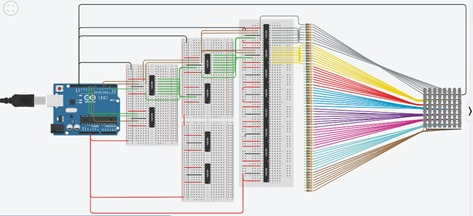
\includegraphics[width=12cm]{Dia 1.jpeg}



\subsection{Día 2}
Cambiamos significativamente el circuito, con el propósito principal de reducir la cantidad de pines usados lo máximo posible y logramos idear uno que solo hace uso de 3 pines, además de librarnos de posibles errores por tanta conexión.\\
Para el algoritmo inicializamos la estructura que íbamos a seguir, las salidas del SER, SRCLK,RCLK y tambíen el puerto serial. Iclusive, realizamos la primera funcion 'Verificacion' con éxito, dándole valores en binario como habíamos acordado antes.\\

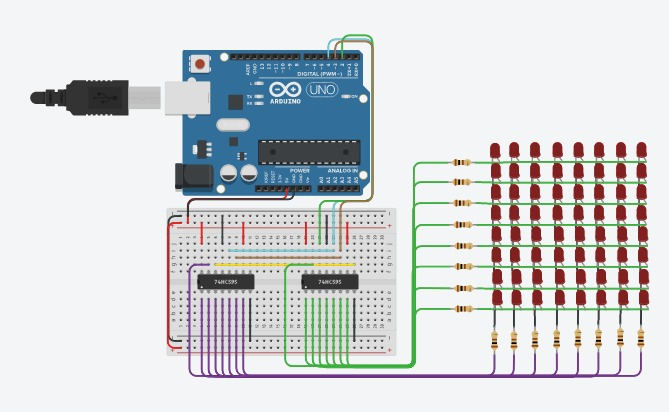
\includegraphics[width=12cm]{Dia 2.jpeg}

\vspace{0.5cm}

Para la función verificacón, que será la base para el resto de funciones, recorrimos las 8 filas de los LED y le asignamos su valor en binario, que en este caso todos bombillos deberían estar encendidos, dentro del arreglo 'ALL' utilizando la función desplazarbyte para leer los bites de cada fila y comprobar si están disponibles\\

\vspace{0.5cm}

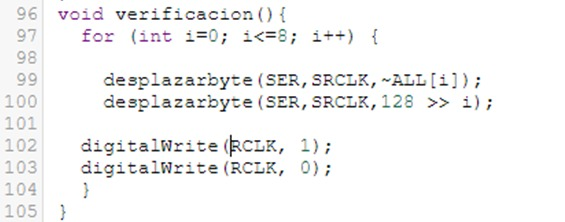
\includegraphics[width=12cm]{Veri.jpeg}

\subsection{Día 3}
Finalmente, avanzamos hasta implementar la función publik a un punto aceptable, con sus respectivas restricciones dadas en la guía. Definimos las funciones para cada letra del abecedario, número decimal y para los emojis dentro de la función imagen para simplificar el trabajo y ser un poco más eficientes, además de agregarle punteros y arreglos\\

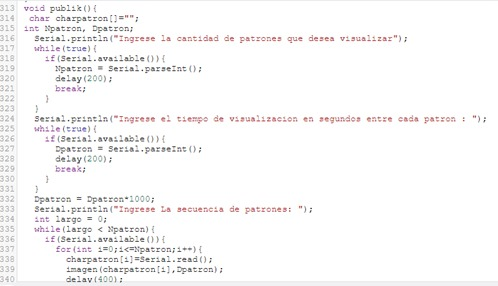
\includegraphics[width=12cm]{Dia 3.jpeg}

\subsection{Día 4}
Realizamos los arreglos finales al código e implementamos memoria dinámica, reestructuración de datos y punteros.

\subsection{Día 5}
Se rediseñaron los caracteres para imprimir en el arreglo 8x8


\label{fig:my_label}
\section{Esquema} \label{contenido}
\begin{figure}
    \centering
    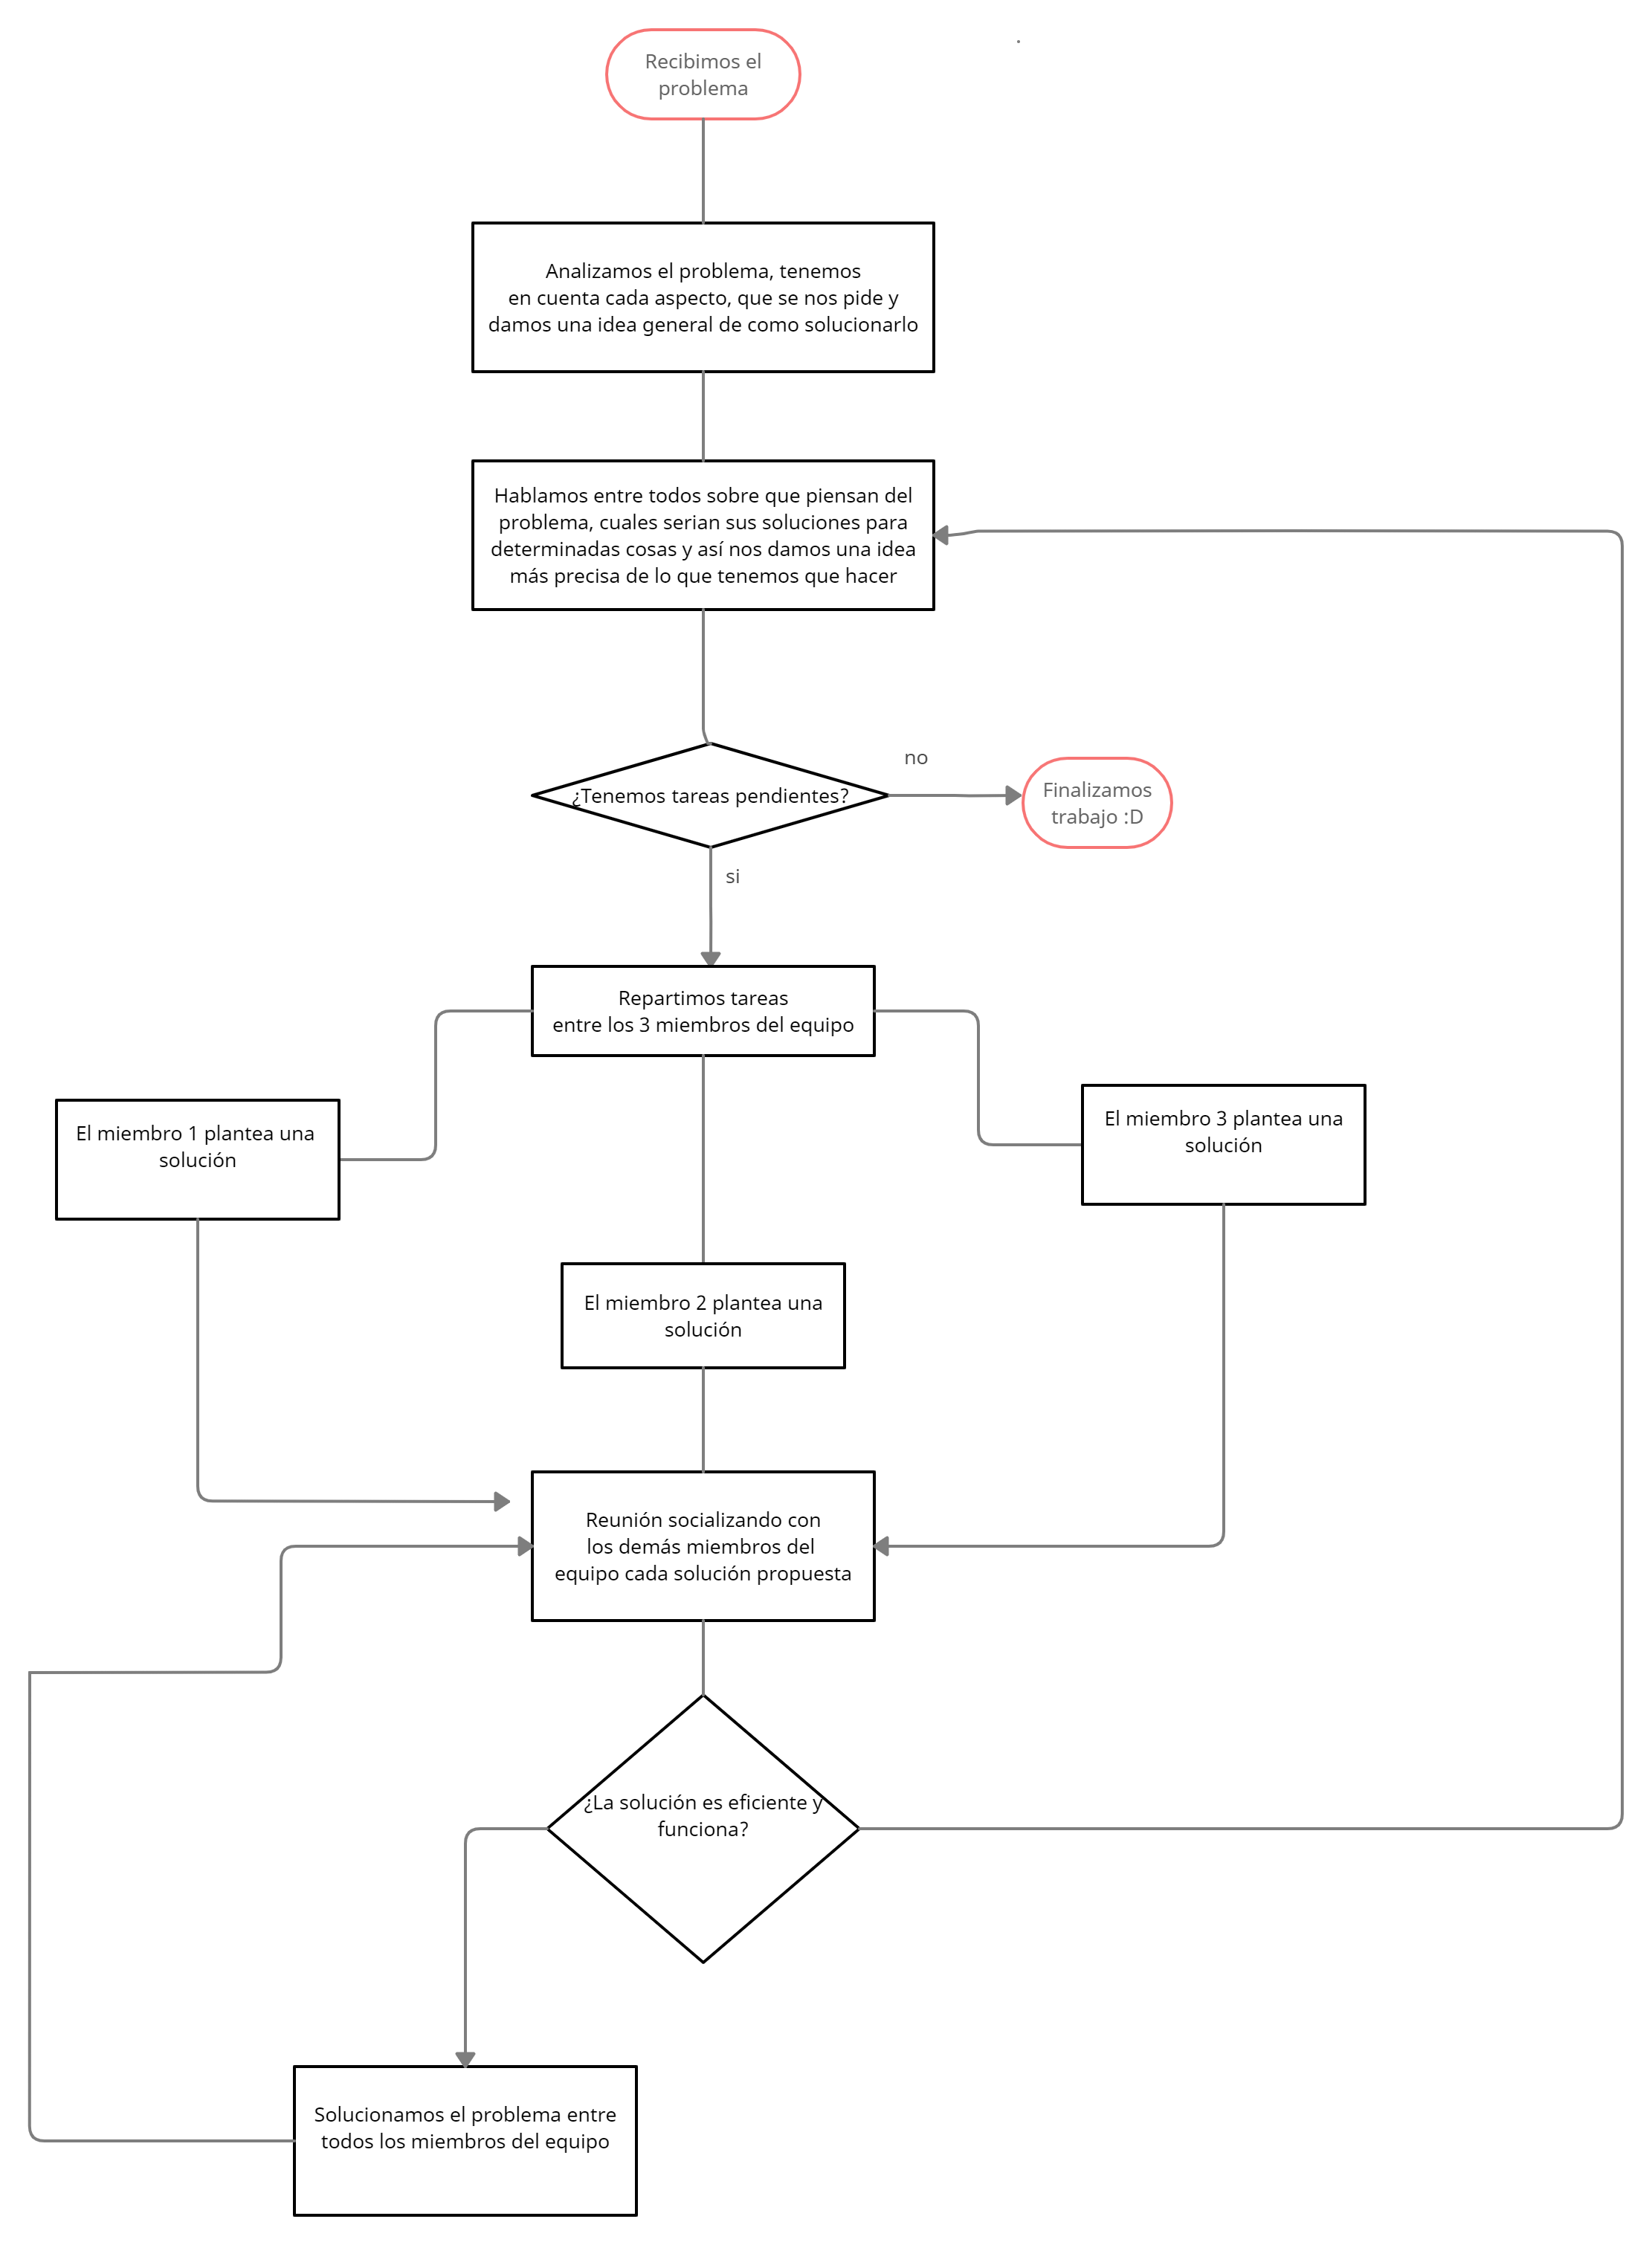
\includegraphics[width=16cm]{diagrama.png}
    \caption{diagrama}
    \label{fig:my_label}
\end{figure}
\bibliographystyle{IEEEtran}
\bibliography{references}

\end{document}